\chapter{Metodologia}

Uma pesquisa científica pode ser classificada quanto à sua abordagem, sua natureza, seus objetivos e seus procedimentos \cite{gerhardt2009tiposdepesquisa}, dessa forma podemos definir que esta pesquisa terá uma abordagem quantitativa, natureza aplicada, objetivo exploratório, e os procedimentos serão de uma pesquisa exploratória.

Esta seção apresenta a metodologia que será empregada no desenvolvimento do trabalho proposto, visando alcançar os objetivos descritos anteriormente.

\section{Rede de Sensores sem Fio}
A rede de sensores proposta coleta dados de temperatura, umidade relativa do ar e molhamento foliar, com o objetivo de, a partir dos dados coletados, efetuar o controle do sistema nebulizador. Os nós presentes na rede estão conectados a Internet por meio de uma rede \textit{WIFI} e a troca de mensagens é realizada utilizando o protocolo MQTT abordado no tópico \ref{sec:mqtt}. A Figura \ref{fig:esquema-rede} mostra um esquema simples de como a rede será organizada.

\begin{figure}[H]
    \centering
    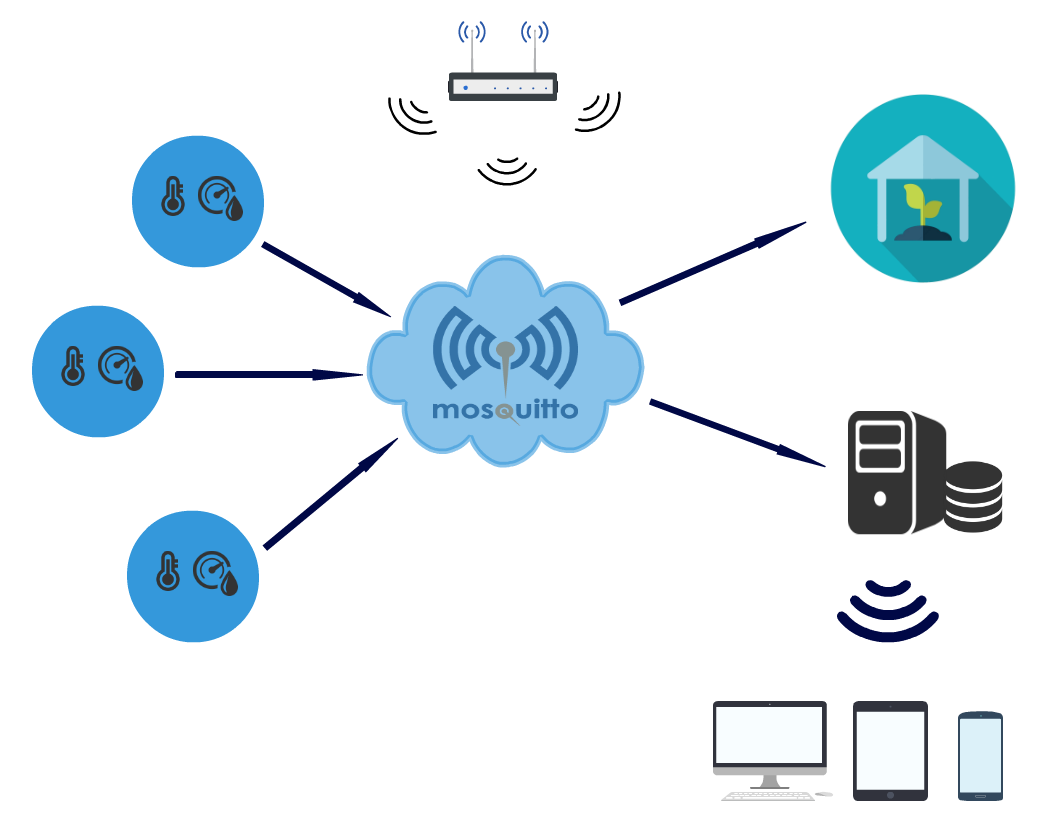
\includegraphics[scale=0.4]{./04-figuras/rede.png}
    \caption{Esquema da rede de sensores.}
    \vspace{-\baselineskip}
    \fonte{Do Autor (2018).}
    \label{fig:esquema-rede}
\end{figure}

A rede se divide em duas partes. A primeira parte se trata do servidor responsável por receber as mensagens publicadas e encaminha-las seus destinos. Neste trabalho foi utilizado o \textit{message broker} Mosquitto\footnote[2]{Para mais informações sobre o \textit{message broker} Mosquito acesse: \url{http://mosquitto.org/}}, que é uma ferramenta \textit{open source} que implementa o protocolo MQTT. A outra parte consiste nos clientes que interagem com o servidor, publicando ou rebendo mensagens.

A programação dos nós foi realizada utilizando-se a linguagem de programação Python\footnote[3]{Para maiores informações sobre a linguagem de programaçao Python acesse: \url{https://www.python.org/}}, o que só foi possível por meio da instalação do \textit{firmware} MicroPython\footnote[4]{Para saber mais sobre o MicroPython acesse: \url{http://docs.micropython.org/en/latest/index.html}} no microcontrolador.

% A rede se divide em duas partes, os nós publicadores, que são os responsáveis por estar efetuando a coleta dos dados dentro da estufa, e os nós assinadores, que se encarregam de receber os dados e efetuar o controle do sistema nebulizador.

\subsection{\textit{Broker} MQTT}
Nesta etapa, inicialmente, foi instalado e configurado o \textit{message broker} Mosquitto em uma máquina virtual Linux disponibilizado pela plataforma Amazon Web Services (AWS)\footnote[5]{Fonte: \url{https://aws.amazon.com/pt/}}, que é uma plataforma de serviços de computação em nuvem.

Após concluídas as configurações foram organizados os tópicos que serão utilizados pelos clientes na troca de mensagens, estes tópicos estão listados na tabela abaixo (Tabela \ref{tab:topicos-mqtt}).

\begin{table}[H]
\centering
\caption{Tópicos utilizados na troca de mensagens.}
\begin{tabular}{p{80pt}|p{300pt}}
\hline
\textbf{Tópico} 			& \textbf{Descrição}\\
\hline
\textit{sensors} 			& Tópico onde são publicados os valores coletados pelos sensores.\\
\hline
\textit{valves/activate}    & Tópico onde são publicadas as mensagens informando se o sistema de nebulização deve ser acionado ou não.\\
\hline
\textit{valves/store}		& Tópico onde são publicadas as mensagens informando se o sistema de nebulização foi acionado para que seja armazenado um \textit{log} de quando ele foi acionado.\\
\hline
\end{tabular}
\label{tab:topicos-mqtt}
\fonte{Do Autor (2018).}
\end{table}


\subsection{Nós Publicadores}
Cada nó é composto por um microcontrolador, e está conectado aos sensores DHT11 (responsável pela coleta de temperatura e umidade relativa do ar) e o sensor de molhamento foliar. A alimentação do nó é realizada por meio de uma bateria de \textit{lithium} com capacidade de 1000mAh. Esta bateria esta conectada ao módulo TP4046, que é alimentado por meio de um painel fotovoltaico, dessa forma, durante o dia a bateria é recarregada.

A Figura \ref{fig:no-publicador} mostra, de forma simples, um esquema de como os componentes estão ligados.

\begin{figure}[H]
    \centering
    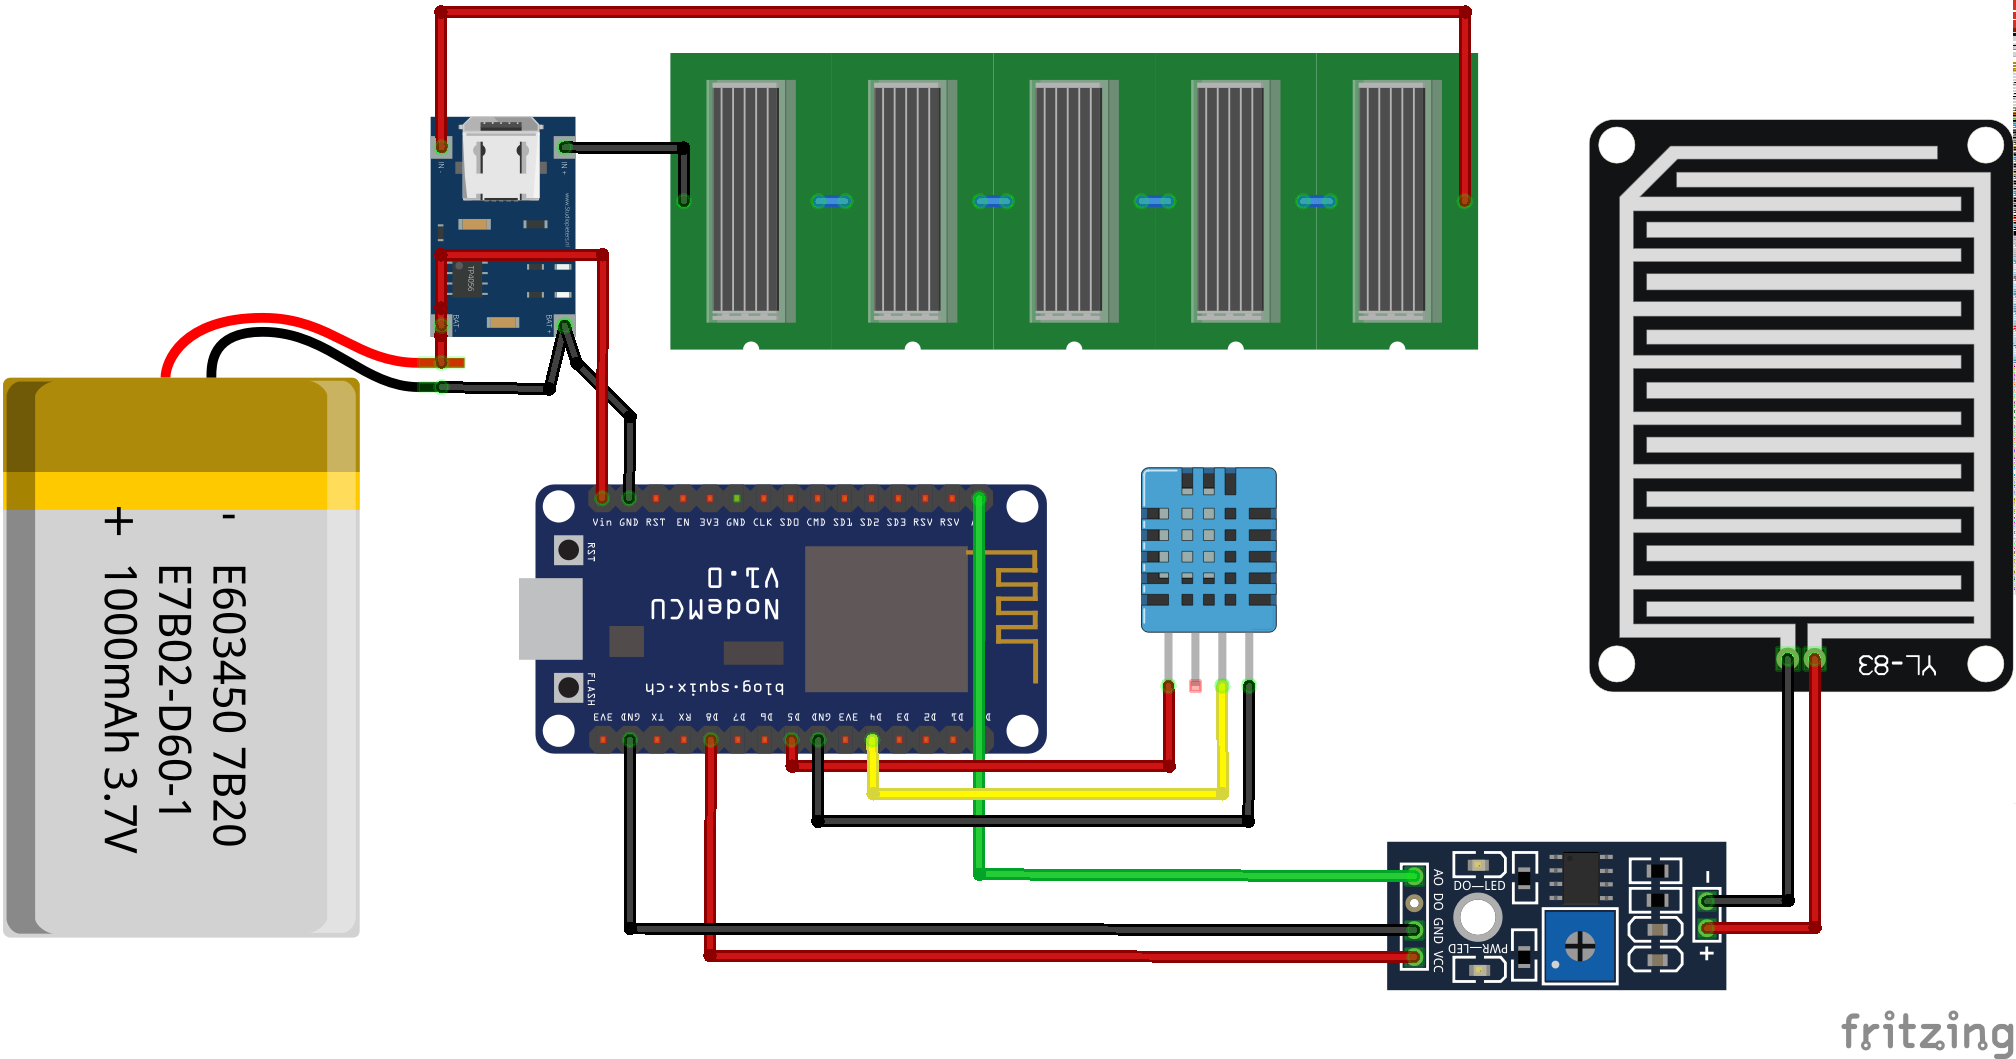
\includegraphics[scale=0.8]{04-figuras/publisher_node.png}
    \caption{Esquema do nó publicador.}
    \vspace{-\baselineskip}
    \fonte{Do Autor (2018).}
    \label{fig:no-publicador}
\end{figure}

Assim que o nó inicia, por padrão, ele executa o código do \textit{boot.py}, neste arquivo foi definido uma função que faz com que o nó busque por todas as redes \textit{WIFI} disponíveis próximas a ele para que possa ser conectar a alguma. Após conectado ele faz uma requisição a um servidor NTP (Network Time Protocol), para realizar a sincronização de data e hora.

O próximo código a ser executado é o arquivo \textit{main.py}, este código contém o \textit{loop} principal do nó, que consiste nas seguintes etapas:

\begin{itemize}
    \item o primeiro passo é efetuar a coleta dos valores lidos pelos sensores;
    \item após coletados estes dados, o nó estabelece uma conexão com o \textit{message broker} Mosquitto para que possa publicar os dados;
    \item se ocorrer algum erro e os dados não forem publicados, o nó efetua o armazenamento destes dados para que eles possam ser enviados posteriormente;
    \item após publicados os dados o nó entra no modo \textit{deep sleep} e permanece "adormecido" pelo intervalo de 3 minutos;
    \item quando o nó despertar ele executará toda a rotina novamente, iniciando pelo arquivo \textit{boot.py} e depois \textit{main.py}, sempre nesta sequencia.
\end{itemize}

A Figura \ref{fig:fluxograma-publicador}, mostra um fluxograma desenvolvido pelo autor para representar a rotina descrita acima.

\begin{figure}[H]
    \centering
    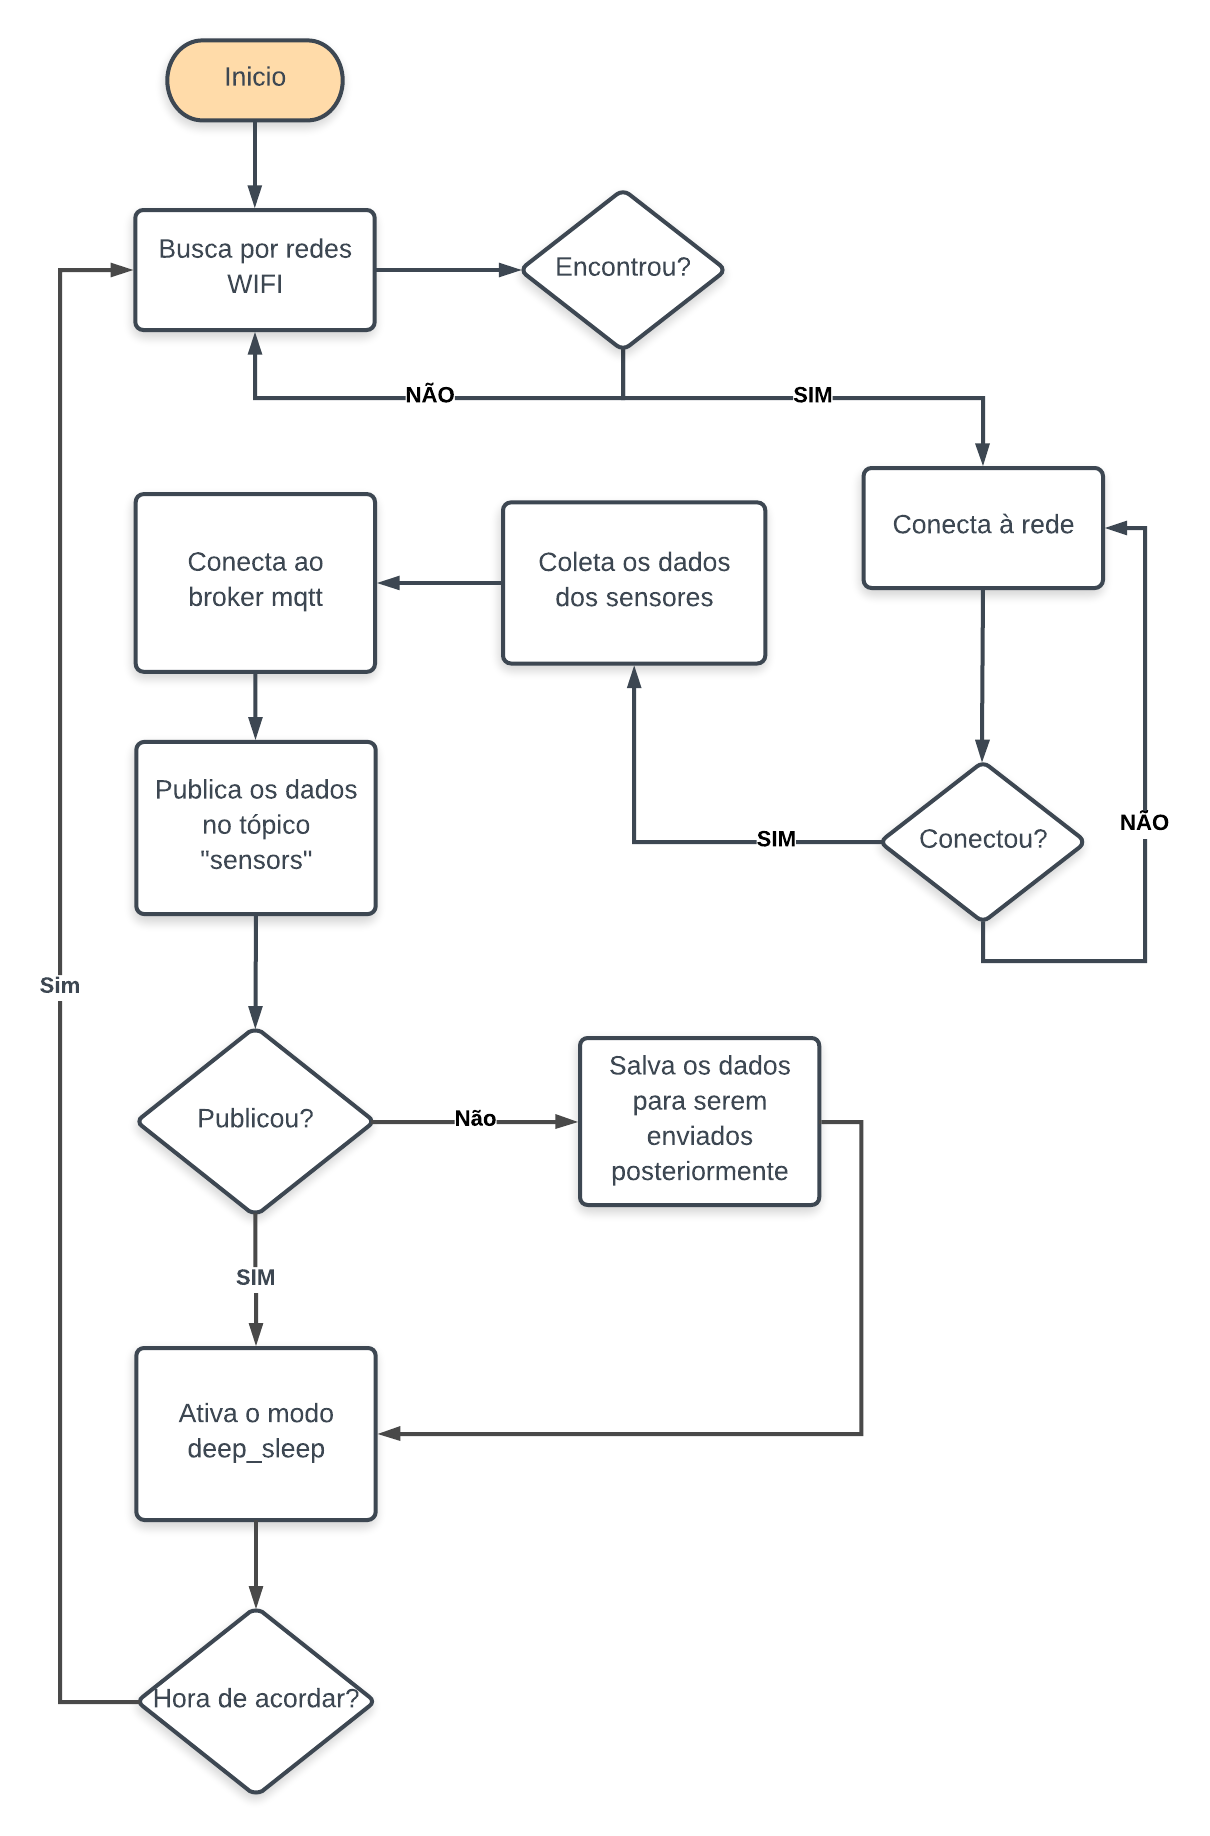
\includegraphics[scale=0.3]{04-figuras/fluxograma-publicador.png}
    \caption{Fluxograma da rotina executada pelo nó publicador.}
    \vspace{-\baselineskip}
    \fonte{Do Autor (2018).}
    \label{fig:fluxograma-publicador}
\end{figure}

As mensagens publicadas por estes nós são compostas por um objeto JSON contendo todas as informações, como monstra o Quadro \ref{tab:formato-mensagens}. A primeira parte da mensagem é formada pelo objeto \textit{"node"} que contém informações relacionadas ao microcontrolador, essas informações são utilizadas para identifica-lo. A segunda parte da mensagem são os valores coletados pelos sensores, são os valores de temperatura, umidade relativa do ar e molhamento foliar. E por final resta o \textit{"timestamp"} que é a chave que armazena a hora em que os dados foram coletados.

\begin{quadro}[H]
\centering
\caption{Formato das Mensagens publicadas no tópico "sensors".}
\vspace{-\baselineskip}
\begin{minted}[
frame=single,
framesep=2mm,
baselinestretch=1.2,
bgcolor=LightGray,
fontsize=\footnotesize,
]{js}
{
    "node": {
        "mac": "",          // Endereço MAC do nó
        "ip": ""            // Endereço IP do nó
    },
    "sensors": {
        "temperature": "",  // Temperatura
        "humidity": "",     // Umidade do ar 
        "leafWetness": ""   // Molhamento foliar
    },
    "timestamp": ""         // Data e hora em que a mensagem foi enviada
}
\end{minted}
\label{tab:formato-mensagens}
\vspace{-1.2cm}
\fonte{Do Autor (2018.)}
\end{quadro}

% Há um nó da rede e um cliente web que estão conectados como assinantes da rede, ou seja, estão escutando todas as mensagens que são publicadas. O nó assinante é responsável por coletar os dados publicados e, a partir deles, tomar decisões quanto ao acionamento do sistema nebulizador. Enquanto, o cliente web é responsável por coletar estes dados e armazena-los em um banco de dados, para que os mesmos possam ser exibidos posteriormente ao usuário por meio de relatórios.

\subsection{Nós Assinadores}
Cada nó é composto pelo microcontrolador esp8266 e um relé de estado sólido, que funciona como uma espécie de interruptor para ligar ou desligar o sistema nebulizador. A alimentação destes nós serão por meio de uma fonte de 5V e 2A.

A figura \ref{fig:no-assinador}, representa um esquema de como estão ligados estes componentes.

\begin{figure}[H]
    \centering
    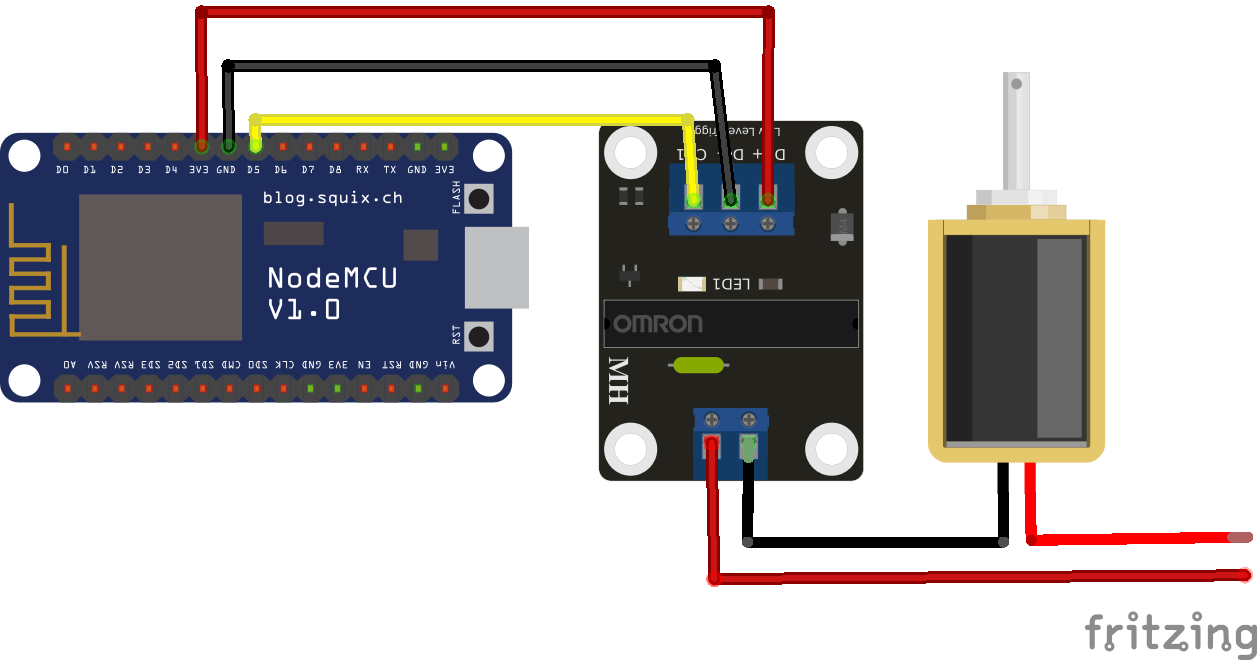
\includegraphics[scale=1]{04-figuras/subscriber_node.png}
    \caption{Esquema do nó assinador.}
    \vspace{-\baselineskip}
    \fonte{Do Autor (2018).}
    \label{fig:no-assinador}
\end{figure}

Da mesma forma que nos nós publicadores, assim que o nó inicia, ele executa o código do \textit{boot.py}, neste arquivo foi definido uma função que faz com que o nó busque por todas as redes \textit{WIFI} disponíveis próximas a ele para que possa ser conectar a alguma. Após conectado ele faz uma requisição a um servidor NTP para realizar a sincronização de data e hora.

A lógica principal do nó e representada pela seguinte rotina (Figura \ref{fig:fluxograma-assinador}):

\begin{itemize}
    \item o primeiro passo é estabelecer uma conexão com o \textit{broker};
    \item após estabelecida a conexão, o nó assina o tópico \textit{"sensors"}, que é onde os nós publicadores estarão publicando os dados coletados;
    \item a cada mensagem recebida, o nó verifica se deve acionar ou não o sistema nebulizador, sendo que, toda vez que o nebulizador é acionado, o nó publica uma mensagem no tópico \textit{"valves/store"} para que seja mantido um registro;
\end{itemize}

\begin{figure}[H]
    \centering
    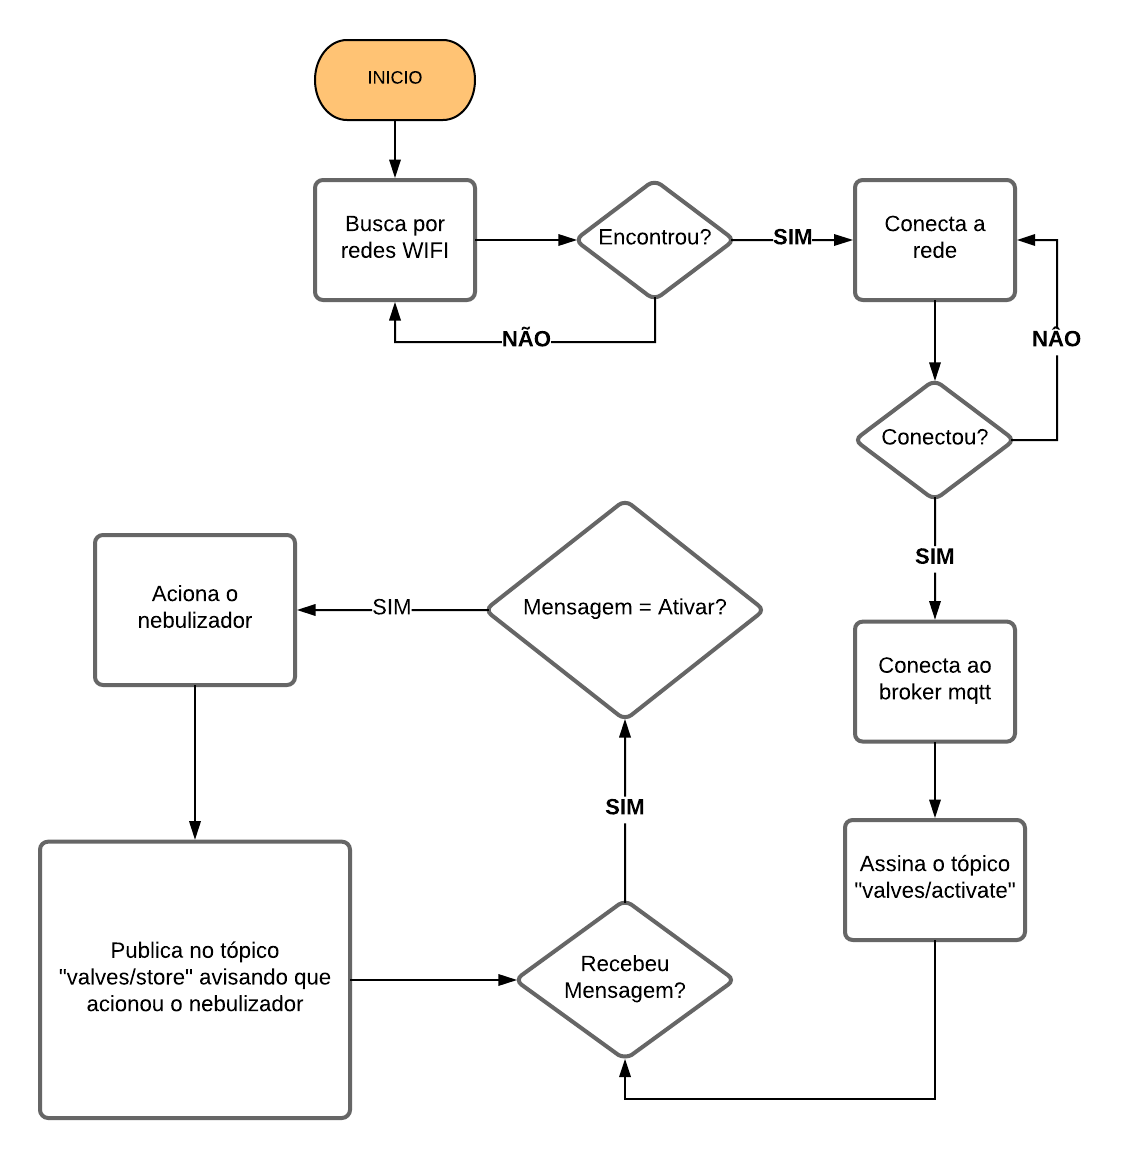
\includegraphics[scale=0.4]{04-figuras/fluxograma-subscriber.png}
    \caption{Fluxograma da rotina executada pelo nó assinador.}
    \vspace{-\baselineskip}
    \fonte{Do Autor (2018).}
    \label{fig:fluxograma-assinador}
\end{figure}

Além desta rotina principal, o nó possui uma rotina de segurança responsável por acionar o sistema nebulizador quando o nó fica a mais de 15 minutos sem receber nenhum dado.

O Quadro \ref{tab:formato-mensagens-assinador} mostra como são as mensagens publicadas por este nó toda vez que o sistema nebulizador for acionado.

\begin{quadro}[H]
\centering
\caption{Formato das Mensagens publicadas no tópico "valves/store".}
\vspace{-\baselineskip}
\begin{minted}[
frame=single,
framesep=2mm,
baselinestretch=1.2,
bgcolor=LightGray,
fontsize=\footnotesize,
]{js}
{
    "location_id": "",    // Id de qual válvula foi acionada
    "measurement_id": "", // Id da medição que deu origem ao acionamento
    "turned_on": "",      // Bit indicando se foi acionado ou não
    "duration": "",       // A duração do acionamento
    "note": ""            // Alguma observação
}
\end{minted}
\label{tab:formato-mensagens-assinador}
\vspace{-1.2cm}
\fonte{Do Autor (2018.)}
\end{quadro}

Há ainda um cliente web que está conectados como assinante do tópico \textit{"sensors"}, ou seja, esta escutando todas as mensagens que são publicadas. Este cliente web é responsável por coletar estes dados e armazena-los em um banco de dados, para que os mesmos possam ser exibidos posteriormente ao usuário por meio de relatórios. Além de também ser o responsável de publicar na rede quando o sistema nebulizador deve ser acionado ou não.


\section{Aplicação Web}
Nesta seção serão apresentados os passos seguidos no desenvolvimento da aplicação, tais como o processo de desenvolvimento de software e tecnologias empregadas.

\subsection{Processo de Desenvolvimento de \textit{Software}} 
O processo de desenvolvimento de \textit{software} utilizado foi o Iterativo e Incremental. Esse processo consiste em um ciclo onde são realizadas tentativas sucessivas de refinamento, a cada iteração são realizadas melhorias no \textit{software}.

\citeonline{bezerra2017iterativoeincremental} define o processo Iterativo e Incremental como um conjunto de ciclos, onde cada ciclo considera um subconjunto de requisitos. Uma vez que estes requisitos são implementados um novo ciclo se inicia, e com este novo ciclo um novo subconjunto de requisitos é considerado para ser desenvolvido, o que produz um novo incremento do sistema. Dessa forma, o desenvolvimento evolui em versões, ao longo da construção incremental e iterativa de novas funcionalidades até que o sistema completo esteja construído.

\begin{figure}[H]
    \centering
    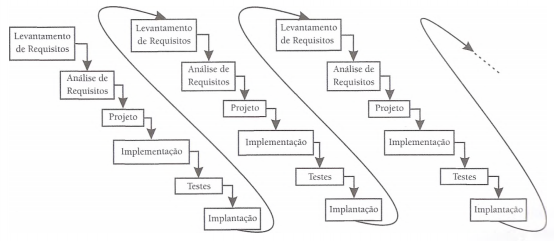
\includegraphics[scale=0.7]{04-figuras/iterativo-incremental.png}
    \caption{Etapas a serem realizadas a cada ciclo.}
    \vspace{-\baselineskip}
    \fonte{\citeonline{bezerra2017iterativoeincremental}.}
    \label{fig:iterativo-incremental}
\end{figure}

Como pode ser observado na figura \ref{fig:iterativo-incremental}, cada ciclo do processo Iterativo e Incremental é composto pelas etapas de análise e levantamento de requisitos, projeto de software, implementação, testes e implantação. \citeonline{bezerra2017iterativoeincremental} ainda afirma que a abordagem incremental estimula a participação do usuário nas etapas do desenvolvimento, o que diminui a chance de ocorrer interpretações erradas em relação aos requisitos levantados, além de também possibilitar um melhor gerenciamento em relação aos riscos do projeto.

\subsection{Levantamento e Análise de Requisitos}
O primeiro passo realizado no desenvolvimento do sistema foi o levantamento de requisitos. Este levantamento foi realizado através de reuniões juntamente ao professor responsável pelo setor de fruticultura. Durante estas reuniões foram definidas as funcionalidades que atendem às necessidades do setor. Após o levantamento ser concluído, foi feito uma análise desses requisitos juntamente ao professor orientador do trabalho, onde foi definido um escopo viável para implementar. 

\subsection{Projeto de \textit{Software}}
Para o projeto de \textit{software} foi utilizada a Linguagem de Modelagem Unificada (UML, do inglês \textit{Unified Modeling Language}), esta linguagem permite a modelagem de sistemas através de elementos gráficos, como diagramas \cite{bezerra2017iterativoeincremental}. 

\begin{figure}[H]
    \centering
    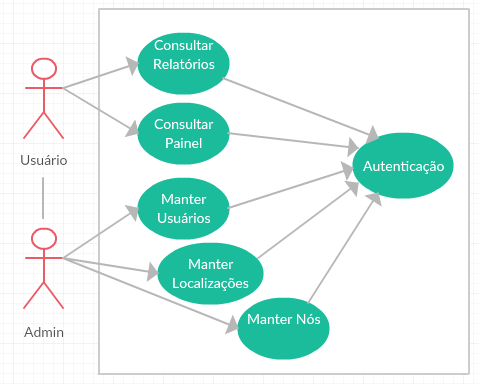
\includegraphics[scale=0.8]{04-figuras/caso_de_uso.png}
    \caption{Diagrama de caso de uso.}
    \vspace{-\baselineskip}
    \fonte{Do Autor (2018).}
    \label{fig:caso-de-uso}
\end{figure}

Nesta etapa foi desenvolvido o diagrama de caso de uso (figura \ref{fig:caso-de-uso}), este diagrama representa a iteração do ator (usuário) com as funcionalidades do sistema através de fluxos \cite{gomes2003casodeuso}.

Como mostra a figura \ref{fig:caso-de-uso}, o sistema conta com dois atores, que representam os
dois grupos de usuários que utilizaram o sistema. O ator "Usuário" tem acesso às funcionalidades de "Consultar Painel" e "Consultar Relatórios", já o ator "Admin", além de herdar estas funcionalidades do ator "Usuário", também possui acesso às funcionalidades de "Manter Localizações", "Manter nós" e "Manter Usuários". Todas as funcionalidades do sistema exigem que o usuário esteja autenticado. O verbo "manter", presente nas funcionalidades, representa quatro operações básicas de banco de dados, \textit{Create, Read, Update e Delete} (CRUD).

\subsection{Implementação}
A implementação do sistema foi dividida em duas partes, \textit{back-end} e \textit{front-end}. O \textit{back-end}, como o próprio nome sugere, é a parte de "trás" da aplicação. É a parte da aplicação que roda no servidor e é responsável pela implementação da regra de negócio. Já o termo \textit{front-end} se refere à parte de interface do sistema, ou seja, é a parte da aplicação que interage diretamente com o usuário.

\subsubsection{\textit{Back-end}}
O \textit{backend} foi desenvolvido utilizando NodeJS\footnote[6]{Mais informações sobre Nodejs podem ser acessadas em: \url{https://nodejs.org/en/}}, que é um interpretador JavaScript \textit{open source} que possibilita a sua utilização como linguagem de servidor, através do \textit{framework web} AdonisJS\footnote[7]{Mais informações sobre Adonisjs podem ser acessadas em: \url{https://adonisjs.com/}}. O desenvolvimento seguirá o padrão \textit{Model, View, Controller} (MVC).

\begin{figure}[H]
    \centering
    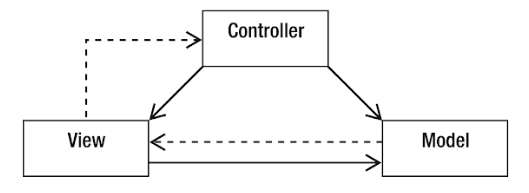
\includegraphics[scale=1]{04-figuras/mvc.png}
    \caption{Arquitetura do padrão MVC.}
    \vspace{-\baselineskip}
    \fonte{\citeonline{dooley2011mvc}.}
    \label{fig:mvc}
\end{figure}

Como podemos ver na figura \ref{fig:mvc}, o padrão MVC se divide em três camadas:
\begin{itemize}[itemsep=0em]
    \item \textit{\textbf{Controller}} (controlador): o controlador interpreta as entradas enviadas pelo usuário e as mapeia em comandos que serão enviados para o modelo e/ou para uma janela de visualização \cite{dooley2011mvc}.
    \item \textit{\textbf{Model}} (modelo): o modelo gerencia os elementos de dados, nesta camada que é realizado a comunicação com o banco de dados  \cite{dooley2011mvc}.
    \item \textit{\textbf{View}} (visão): visão é a camada responsável por apresentar os dados ao usuário \cite{dooley2011mvc}.
\end{itemize}

Como banco de dados foi escolhido o MySQL, que é um sistema de gerenciamento de banco de dados que utiliza a linguagem SQL como interface, além se ser atualmente um dos sistemas de gerenciamento de bancos de dados mais populares.

\vfill

\subsubsection{\textit{Front-end}}
O \textit{front-end} do sistema foi desenvolvido utilizando a linguagem JavaScript por meio da biblioteca ReactJS. Esta biblioteca foi desenvolvida pela equipe de desenvolvedores do Facebook e Instagram, é uma biblioteca que funciona na ideia de componentização, onde a ideia é quebrar os elementos em pequenos componentes reutilizáveis. Para desenvolvimento da interface foram empregados os conceitos de \textit{Material Design} por meio do \textit{framework} Material UI que implementa esse conceito.

\subsection{Testes e Implantação}
Nesta etapa do desenvolvimento serão realizados testes automatizados nas funcionalidades do sistema. Após testadas as funcionalidades serão efetuados testes de usabilidade da aplicação buscando um \textit{feedback} do usuário para que o sistema possa ser melhorado. Realizado os devidos testes se dará inicio a mais um ciclo de desenvolvimento, este ciclo se repetirá até que o sistema completo esteja concluído e valido para que possa ser implantado.

\section{Experimentos}
Nesta etapa serão efetuados experimentos visando verificar se o trabalho desenvolvido cumpre a proposta de trazer melhorias na produção. Serão separados dois ambientes distintos:

\begin{itemize}[itemsep=0em]
\item O primeiro ambiente estará sob as condições atuais onde o sistema nebulizador é acionado de maneira estática.
\item O segundo ambiente estará sendo controlado pelo sistema desenvolvido.
\end{itemize}

Serão colocadas mudas nos dois ambientes para que possa ser avaliado sob quais condições será obtido o melhor resultado.